\documentclass{sig-alternate}
\usepackage{amsmath}
\usepackage{amssymb}
\usepackage{times}

\usepackage{enumerate}
\usepackage{subfigure}
\usepackage{graphicx}

\usepackage{comment}
\usepackage{cite}
\usepackage{epstopdf}

\pdfpagewidth=8.5in
\pdfpageheight=11in

\makeatletter
\newif\if@restonecol
\makeatother
%
\let\endalgorithm\relax
\usepackage[linesnumbered,ruled,vlined]{algorithm2e}

\newcommand{\reminder}[1]{ [[[ \marginpar{\mbox{$<==$}} #1 ]]] }
\newcommand{\GC}[1]{\reminder{{\bf Gao}: #1}}

\newcommand{\kw}[1]{{\ensuremath {\mathsf{#1}}}\xspace}
\newcommand{\MatchDist}{\mbox{\sf Match}\xspace}
\newcommand{\AnchorMatchDist}{\mbox{\sf AnchorMatch}\xspace}
\newcommand{\PartialEval}{\mbox{\sf PartialEval}\xspace}
\newcommand{\IsMatch}{\mbox{\sf IsMatch}\xspace}
\newcommand{\matchDist}{\mbox{\sf matchDist}\xspace}
\newcommand{\minMatchDist}{\mbox{\sf minMatchDist}\xspace}
\newcommand{\Dist}{\mbox{$\mathsf{Dist}$}\xspace}
\newcommand{\minDist}{\mbox{$\mathsf{minDist}$}\xspace}
\newcommand{\Cost}{\mbox{$\mathsf{Cost}$}}
\newcommand{\Group}{\mbox{$\mathsf{Group}$}}


\newcounter{example}[section]
\renewcommand{\theexample}{\nthesection.\arabic{example}}
\newenvironment{example}{
    \refstepcounter{example}
    {\vspace{1ex} \noindent\bf  Example  \theexample:}}{
    \eop\vspace{1ex}} %\hspace*{\fill}\vspace*{1ex}}


\newcounter{theorem}[section]
\renewcommand{\thetheorem}{\nthesection.\arabic{theorem}}
\newenvironment{theorem}{\begin{em}
    \refstepcounter{theorem}
    {\vspace{1ex} \noindent\bf  Theorem  \thetheorem:}}{
    \end{em}\eop\vspace{1ex}} %\hspace*{\fill}\vspace*{1ex}}
\renewenvironment{proof}{
    {\vspace{1ex} \noindent\bf  Proof:}}{
    \eop \vspace{1ex} }

\newenvironment{lemma}{\begin{em}
    \refstepcounter{theorem}
    {\vspace{1ex} \noindent\bf  Lemma  \thetheorem:}}{
    \end{em}\eop\vspace{1ex}} %\hspace*{\fill}\vspace*{1ex}}


\newcommand{\nthesection}{\arabic{section}}
\newcommand{\eop}{\hspace*{\fill}\mbox{$\Box$}}
\newcommand{\eat}[1]{}
\newcommand{\stitle}[1]{\vspace{0.5ex}\noindent{\bf #1}}

\renewenvironment{proof}{
    {\vspace{1ex} \noindent\bf  Proof:}}{
    \vspace{1ex} }

\newtheorem{defi}{Definition}

\begin{document}
\conferenceinfo{SIGMOD'11,} {June 12--16, 2011, Athens, Greece.}
\CopyrightYear{2011}
\crdata{978-1-4503-0661-4/11/06}
\clubpenalty=10000
\widowpenalty = 10000
%
% --- Author Metadata here ---
%\conferenceinfo{ACM SIGMOD}{'09 Providence, Rhode Island USA}
%\CopyrightYear{2001} % Allows default copyright year (2000) to be over-ridden - IF NEED BE.
%\crdata{0-12345-67-8/90/01}  % Allows default copyright data (0-89791-88-6/97/05) to be over-ridden - IF NEED BE.
% --- End of Author Metadata ---

\title{Collective Spatial Keyword Querying}
%
% You need the command \numberofauthors to handle the "boxing"
% and alignment of the authors under the title, and to add
% a section for authors number 4 through n.
%

%%%%%%%%%%%%%%%
%%%%%%%%%%%%%%%
%%%%%%%%%%%%%%%
%%%%%%%%%%%%%%%


\maketitle


\section{PROCESSING TYPE2 SPATIAL GROUP KEYWORD QUERIES} \label{sec:type2}
\subsection{Circle Range Limitation} \label{secsub:type2:limitation}
Recall the defination of \textsf{TYPE2} problem. The total cost is determined
by two part, and the first part depends on the furthest object while
the second part depends on all pairs of all feasible objects.
For ease of presenting our method, we set parameter $\alpha$ into 0
to disregard the first part cost and discuss the difference
in section ?? when considering this parameter.\par
%
For some given objects, it's possible to find a \textsf{Smallest Enclosing Circle}
which covers all the objects and has the diameter as small as possible. A circle is
helpful for us to make some limitation, because it's obvious that the distance of
any two objects won't exceed the diameter of this smallest enclosing circle $D$.
Therefore, a circle limitation is helpful for us to approach the exact result
of \textsf{TYPE2} problem which is challenging to find the diameter of the keywords-covered
objects. In order to avoid the obscurity of two diameter defination, we call the
diameter of the enclosing circle $D$ and the diameter of the inside objects $L$.\par
%

For known objects it's always possible to find such a circle limitaion,
nevertheless, the problem in \textsf{TYPE2} is the inverse process which aims to
select a subset of all objects with a circle limitaion and covers all the
keywords as well. Figure~\ref{fig:1} shows an example of smallest enclosing circle.

\begin{figure}\label{fig:1}
\begin{center}
\centering
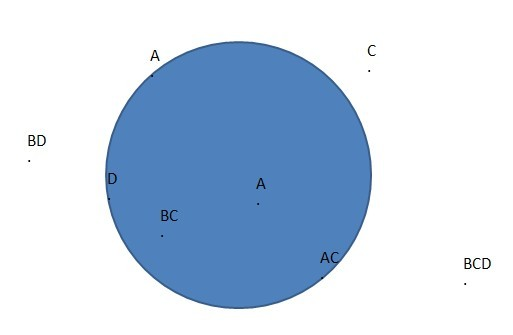
\includegraphics[width=2.5in]{figure/fig1}
\caption{An example of Smallest Enclosing Circle with query \{A,B,C,D\}.}
\end{center}
\end{figure}

\begin{theorem}\label{thm:lambda}
For a set of given points $P$ on the 2-dimensional plane,
the diameter of $P$ is $L$ and the diameter of
$P$'s smallest enclosing circle is $D$. If $|P|>1$ we have
the limition relationship: 
$ \frac{\sqrt{3}}{2} \cdot D\leq L \leq D$

\proof
Some proof here
\end{theorem}

The value of $\frac{\sqrt{3}}{2}$ will be mentional repeatedly,
so we use $\lambda$ to substitute this constant.
According to the above property, it's more clear if we
have the inequality changed into: $L \leq D \leq \frac{L}{\lambda}$.
This means if we find a circle with diameter $D$ and with
feasible objects inside we can make sure that
the result of diameter $L$ must be $[\lambda\cdot D,D]$
without any calculation. Namely, the upperbound and lowerbound
can be utilized to prune in the search space when even
the best lowerbound value can't lead to a better solution.

\begin{lemma}\label{lemma:monotone}
The value of diameter $D$ corresponding to the optimal solution
is monotonous. That is, if the circle covering the optimal solution
with a diameter $D$ we can always find a bigger circle with
diameter $D'(D' > D)$ that covers the optimal solution.

\proof
If set $S$ is the optimal solution of \textsf{TYPE2} problem,
we could find it's smallest enclosing circle $C$ with a diameter $D$.
The circle $C'$ with diameter $D'$ could fulfill the condition
if put outside the circle $C$.
\end{lemma}

An obvious opinion according to Lemma~\ref{lemma:monotone} is that
we devote to find a circle which both covering all the query keywords 
and with a diameter as small as possible. But according to
Theorem~\ref{thm:lambda} the reverse process is not absolutely
correct if we believe that the circle with the smallest diameter
will cover the optimal feasible solution. We will discuss this problem
and show how to fix it in the next part.

\subsection{Sweeping Circle} \label{secsub:type2:sweeping}
We just showed that a circle would help us to limit the objects
in some specific area. It's still challenging to find a concrete
position of the circle. We know that three points on the 2-dimensional plane
can determine a circle, but for the smallest enclosing circle problem we
have an analogous conclusion.
%

\begin{lemma}\label{lemma:boundary}
For a set of given points $P(|P|>1)$ on the 2-dimensional plane,
at least two points in $P$ are on the boundary of the smallest enclosing circle.

\proof
Let's utilize reduction to absurdity to prove. Suppose that only one point 
$P_i$ in $P$ is on the boundary of the circle $C$. If the diameter of $C$
is $D$, an $\epsilon$ exists such that a circle $C'$ with diameter $D-\epsilon$
and $C'$ is tangent to $C$ at point $P_i$. If any point is outside the
circle $C'$, we can decrease $\epsilon$ until all the points of $P$ inside
$C'$. Due to $D-\epsilon < D$, $C'$ is smaller than $C$ so $C$ is not
the smallest enclosing circle.
\end{lemma}

\begin{figure}\label{fig:5}
\begin{center}
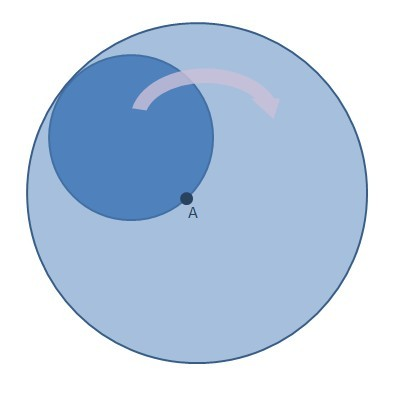
\includegraphics[width=1.5in]{figure/fig5}
\caption{Sweeping Circle Method Schematic Diagram}
\end{center}
\end{figure}

Now we can fix a point on the boundary of the circle based on Lemma~\ref{lemma:boundary}.
There is also an $O(nlogn)$ algorithm to calculate the diameter of given points 
which utilizes \textbf{Rotating Callipers in Convex Hull}. In the rotating callipers
algorithm, a convex hull is computed and two horizontal lines are defined
that enclose the points. Then rotate the lines together while proceeding along the
convex hull. In our problem we enumerate an object to be fixed and have the
diameter-determined circle rotated. If in a rotating angle all the objects inside
this circle cover all the query keywords, we can make sure that at least one feasible solution
exists among these objects. As we enumerate all the objects to be the fixed
one, even for the best solution one object must be on the boundary of the sweeping circle
according to Lemma~\ref{lemma:boundary}. Figure~\ref{fig:5} reflects the sweeping circle method.
Given the fixed object and a proper circle diameter $D$,
the best solution must be cover by the sweeping circle at a specific angle.
%

The sweeping circle strategy is based on an assumption that the circle diameter $D$
is given. Now let's discuss how to determine the value of $D$ to get the
correct optimal results as well as avoiding useless enumeration with efficiency.
%

First, the correctness must be guaranteed. As we have introduced before, a smaller
diameter seems always better by intuition but whether the minimun diameter would 
not miss the optimal objects and guarantee the minimun value $L$?
%

\begin{figure}\label{fig:2}
\begin{center}
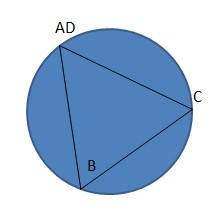
\includegraphics[width=1.5in]{figure/fig2}
\caption{Extreme case of diameter lower bound.}
\end{center}
\end{figure}

\begin{figure}\label{fig:3}
\begin{center}
\centering
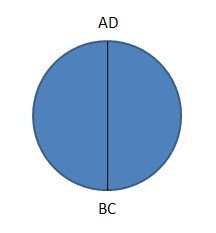
\includegraphics[width=1.5in]{figure/fig3}
\caption{Extreme case of diameter upper bound.}
\end{center}
\end{figure}

\begin{example}\label{ex:counter}
Consider this situation as Figure~\ref{fig:2} and Figure~\ref{fig:3} shows:
Figure~\ref{fig:2} shows the furthest objects pair is exactly the diameter
of enclosing circle. Figure~\ref{fig:3} shows the three objects form an equilateral triangle.
Here we have $L_1 = \lambda\cdot D_1$ and $L_2 = D_2$ which reflects two extreme cases
of Theorem~\ref{thm:lambda} respectively. But if $L_1 < L_2$ and $D_1 > D_2$, we get
$\lambda\cdot D_1 < D_2 < D_1$ which is totally rational.
If we consider $D_2$ to be the lower bound to find the optimal solution,
we would miss $L_1$ which is a better result.
\end{example}
%

Example~\ref{ex:counter} shows a counter-example of considering the minimun
of diameter $D$ would cover the optiaml solution.

\begin{lemma}\label{lemma:enlarge}
Suppose $D$ to be the lower bound of diameter that could cover a feasible
set of objects. Sweeping circle with a diameter of $\frac{D}{\lambda}$ could
cover the optimal solution at some specific position.

\proof
Formally, let $L$ be the optimal distance of furthest pair objects,
and $L'$ be the second optimal one. We have $L \leq L'$.

According to Theorem~\ref{thm:lambda}, $L\leq D \leq \frac{L}{\lambda}$
where $D$ corresponds to the smallest enclosing circle.

Some proof here~
\end{lemma}



\begin{algorithm}[!ht]\small\label{alg:binarysearch}
\caption{ \bf {Framework of Binary Search} (objects,eps)}

$low \gets 0$\;
$high \gets \infty$\;
\While{$high - low > eps$}{
	$D \gets (high + low)/2$\;
	$is\_any\_objects\_possible \gets false$\;
	\For{each object in objects}{
		\If{$circle\_scan(object,D,false)$}{
			$is\_any\_objects\_possible \gets true$\;
			break\;
		}
	}

	\eIf{$is\_all\_objects\_possible$}{
		$high \gets D$\;
	}{
		$low \gets D$\;
	}
}
$D \gets D/\lambda$\;
\For{each object in objects}{
	$circle\_scan(object,D,true)$\;
}
\Return $D$\;\vspace{-1ex}

\end{algorithm}

















\end{document}
